
\section{The Swiss Post addresses data quality in multiple ways}
\label{SolutionMultipleTeams}
At the start of this project, the objective was to develop a minimal viable product (\gls{MVP}) to replace a manual data quality check performed by the business with a more robust solution, including automation, the delivery of reports, as well as an appropriate notification and alerting. However, after beginning this project, Swiss Post management assigned a new priority to the topic of data quality management (\gls{DQM}) overall; therefore, quite unexpectedly, this project acquired an additional set of key stakeholders, located in different teams as discussed in chapter \ref{sec:AWSmodernisationteam}. 


Fortunately, this project as originally conceived fit very well into the larger \gls{DQM} picture.  Coordination with these teams although not originally envisioned (such as the DQM team described in chapter \ref{sec:DQMteam}) therefore became an important task. This coordination was essential for several reasons: first and most obviously,  the project must avoid reinventing existing solutions or overlapping in an unplanned way with other new initiatives. Second, it must ensure that methods and deliverables of this project conform to any new data architecture standards; for example, data quality dimensions have already been defined and documented by other teams. Finally, it must ensure that ongoing work by other teams is taken into account. 



\section{Rule-Based DQM Initiative}
\label{DQMRuleBasedInitiative}

The current architectural goal pursued by the \gls{DQM} team is shown in the following visualisation. The rule evaluation engine, shown at the top centre, executes defined rules on target data and stores the corresponding rule results in a database. In this context, a rule represents a data quality check for a defined dataset, and many different rules can be defined. These rules may, for example, specify allowed values, such as restricting the gender attribute to the three values \textit{male}, \textit{female}, and \textit{not stated}. Alternatively, they may define expected data types, such as requiring dates to be stored in UTC format, or specify valid value ranges depending on the weekday.

Although the rule evaluation engine was a major topic during the weekly exchanges with the \gls{DQM} team, it was not implemented by the project team. Nevertheless, its development progress was regularly monitored and discussed during these meetings. Furthermore, the \gls{ASTV} team used this tool for its intended purpose. However, this usage was outside the scope of this project.


\begin{figure}[H]
    \centering
    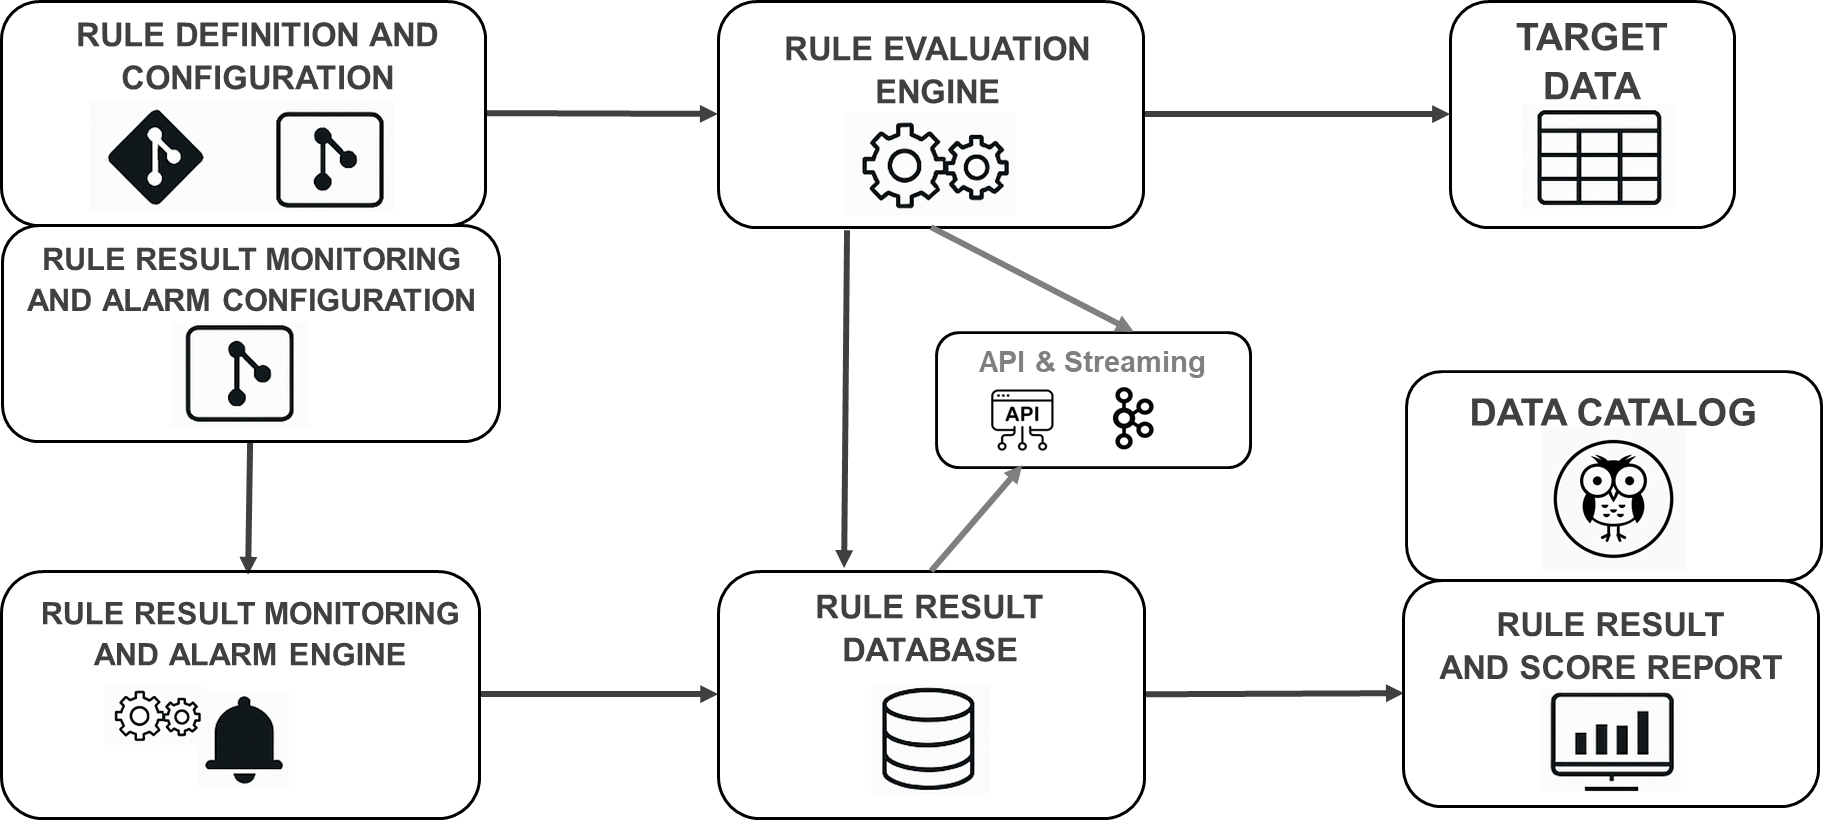
\includegraphics[width=0.8\textwidth]{./content/img/ProjectManagement/dqm_rules_architecture.png}
    \caption{The rule check engine architecture for future DQM}
    \label{fig:dwhlsops_kpi14_future_rulecheck_dqm}
\end{figure}



\subsection*{High-Level Target}
\label{SolutionDQMTeamHighLevelTarget}

From the complete target solution architecture, the first component to be implemented is a rule-based DQM suite. Its objective is to define generic data quality checks that can be applied across different datasets. This is achieved either by abstracting the check from the underlying data or by providing an SQL query that returns the data in a format allowing the same check to be applied to different datasets. The technology used to implement this solution is not discussed in this document, as the implementation was carried out by another team and is therefore outside the scope of this project. This approach consists of four main steps:

\begin{itemize}
    \item \textbf{Configuration}: Configuration defines the tables to be checked, the execution frequency, and the type of check.
    \item \textbf{Data preparation}: An SQL query prepares the data in a format suitable for the check.
    \item \textbf{Rule execution}: An application executes the defined checks on the prepared data.
    \item \textbf{Result persistence}: The results are stored in a database, which enables reporting.
\end{itemize}

\begin{figure}[H]
    \centering
    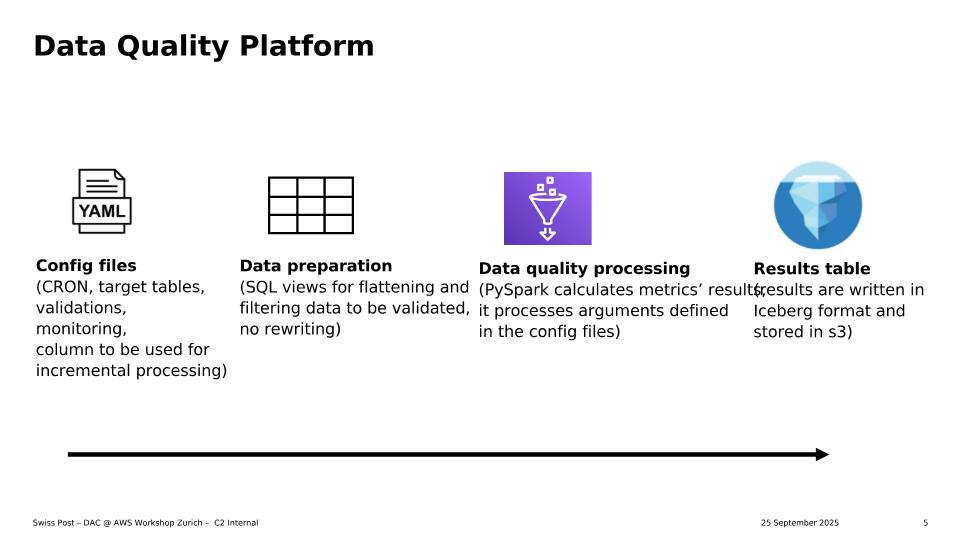
\includegraphics[width=0.8\textwidth]{./content/img/Solution_Design/Slide5.jpg}
    \caption{Intention of a DQM platform, high level}
    \label{fig:solutiondesign_slide5}
\end{figure}



\subsection*{Discarded Solutions}

This initiative is of high importance to the project, as it creates a major organisation-wide constraint to follow the \gls{DQM} team's choice of tool. The rationale for developing a rule-based DQM solution is that existing tools, such as \gls{AWSGlueDQ}, do not support views with complex data types, while \gls{PyDeequ} does not provide row-level results. These limitations in the evaluated tools led to the decision to develop a dedicated solution at Swiss Post, as described above. The following section provides a brief overview of the tools and approaches that were evaluated but ultimately discarded as unsuitable. The following screenshot shows the presentation in which the \gls{DQM} team summarised the evaluated tools and explained the reasoning behind their decision.


\begin{figure}[H]
    \centering
    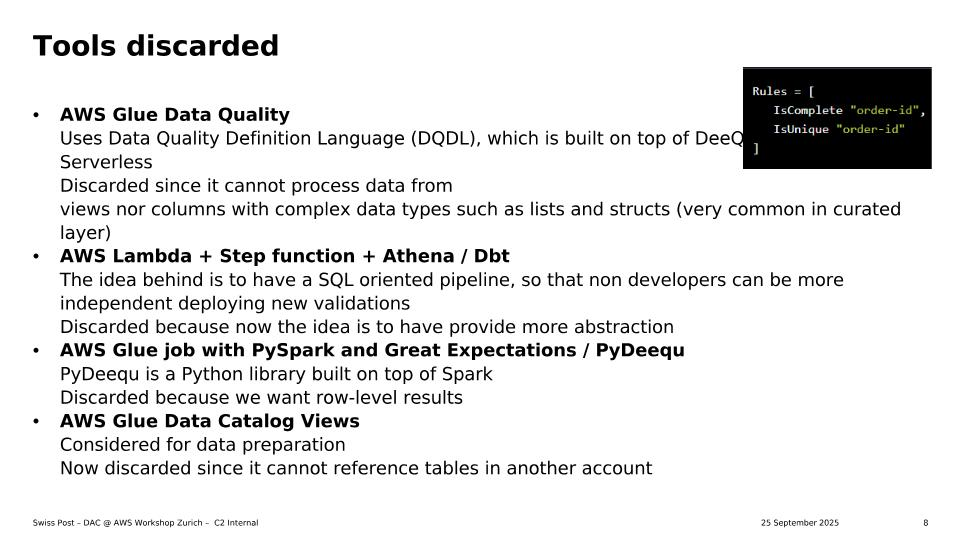
\includegraphics[width=0.8\textwidth]{./content/img/Solution_Design/Slide8.jpg}
    \caption{The list of tools discarded and the reasons for their exclusion}
    \label{fig:dwhlsops_kpi14_discarded_solutions}
\end{figure}

\subsection*{State at the end of this project}
\label{SolutionDQMEndOf2025}
By the end of 2025, the \gls{DQM} team set up a PoC of the rule check engine based on the design shown at the start of this section \ref{fig:dwhlsops_kpi14_future_rulecheck_dqm}. It allows running a check on a database view for specific target data source and storing the rule results in a designated rule result database. However many details were still not defined or implemented. Such as the location where the results check database is to be installed which has not been defined. Also the alerting and the setup of dashboards are currently out of scope, as are later additions such as deriving expected value ranges from historical data or holiday calendars. 



\section{Heterogenous sorting center environments}
\label{SolutionLandscapeMultHardWlayouts}
Before turning to the data lineage, an important constraint must be highlighted. The hardware used by Swiss Post in their high-tech “cyber” postal sorting centers differs in two main ways: across different providers and across different sizes and organisational structures of sorting centers. Which, in turn, also led to a diversity of processes to perform similar actions. This diversity on different levels brings certain benefits but also introduces additional synchronisation effort in other areas.

\subsection*{Different sorting hardware providers}
The hardware used by Swiss Post in its sorting centers is sourced from different providers. This is an essential risk management measure to reduce dependency on a single vendor. To mitigate this risk, Swiss Post decided to rely on at least two providers for essential hardware, not only to avoid dependency but also to protect against delivery issues or even the bankruptcy of individual providers. From a risk management perspective, this approach supports business continuity. However, from an IT perspective, it introduces challenges, as different hardware providers deliver data in different formats or with varying characteristics.

\subsection*{Different sorting center sizes and structure}
The Swiss Post parcel sorting centers are distinguished into two categories. There is one large \gls{PC} parcel center per \gls{region}, which is supplemented by smaller \gls{RPC} regional parcel centers. Regions encompass multiple cantons and may split cantons into the four current regions: west, middle, east, and south. The organisation into larger parcel centers and smaller regional parcel centers helps to optimise processes and reduce the carbon footprint of postal services. However, each PC and RPC differs from the others.

First, due to differences in size, processes differ between small and large centers, and the way of work also varies as organisational structures are different. Second, beyond the distinction between small and large centers, each center has a unique layout. Third, tasks can differ between centers; for example, some also handle letters. While these differences are reasonable from an operational perspective, they introduce challenges for centralised reporting, where all variations need to be harmonised. The following figure shows selected PC and RPC locations distributed across Switzerland.

\begin{figure}[H]
    \centering
    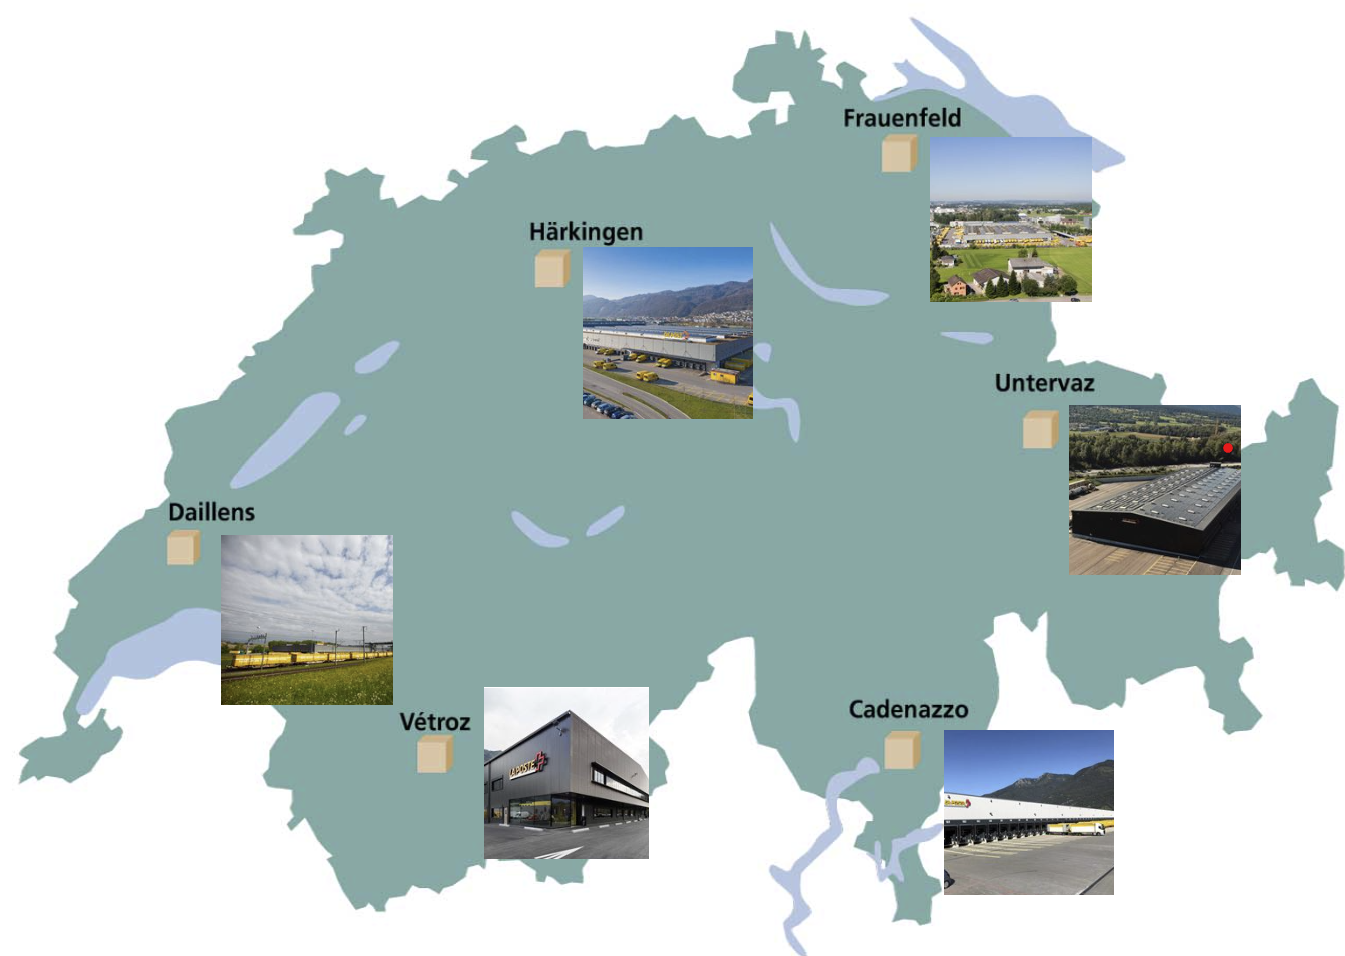
\includegraphics[width=0.8\textwidth]{./content/img/Solution_Design/PZ_RPZ_Schweiz_Edit.png}
    \caption{Selection of parcel sorting centers distributed over Switzerland}
    \label{fig:design_PC_and_RPC}
\end{figure}

\subsection*{Different sorting processes}
\label{SolutionLandscapeLayoutsDiffProcess}
To go one step further, the different size and equipment at the sorting centers lead to different actions performed in the sorting centers. The same event in a sorting center can be caused by different previous actions making reporting on them difficult. As an example, the submitted and discharged events are described further.

\subsubsection*{Submitted event}
\label{SolutionSubmittedEvent}
The submitted event is the first automatic scan that occurs after a mail piece is placed onto the automatic sorting machine. In the context of this project, a mail piece refers to a parcel. However, parcels are not always placed onto the sorting machine in the same way. This can occur via roll boxes (\gls{RX}), which are automatically emptied by robots. An RX is a container, as depicted in the following figures, that is used to transport different mail pieces through sorting and delivery facilities. Alternatively, parcels can be placed onto the automatic machine manually by staff, either by removing them from RX units or by emptying truck containers onto conveyor belts, as shown in the subsequent figures.

\begin{figure}[H]
    \centering
    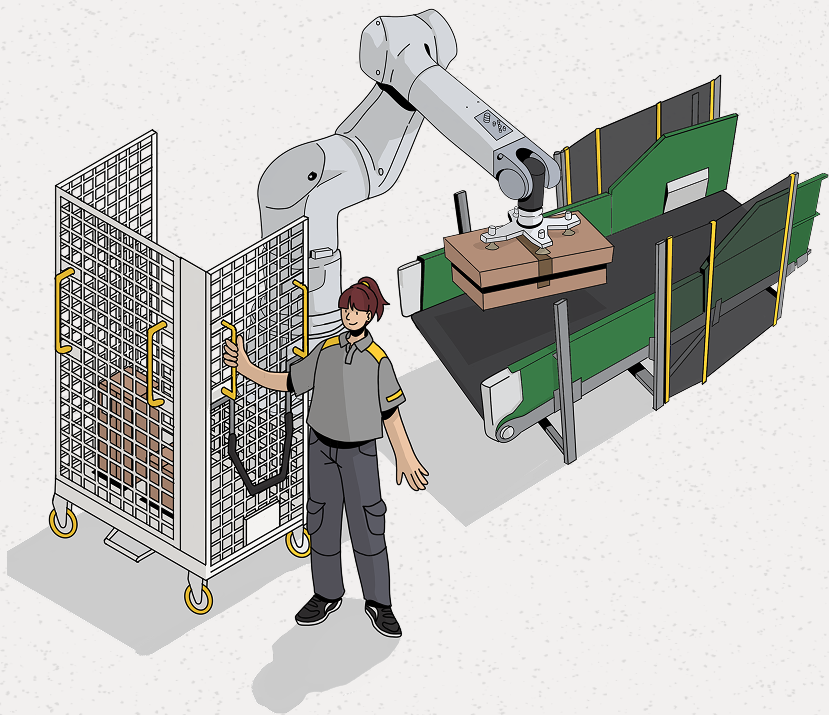
\includegraphics[width=0.8\textwidth]{./content/img/Post_internal/Visual_Subm_PostGraphic_02_12_2025.png}
    \caption{Parcel sorting, parcels submitted by robot}
    \label{fig:submitting_robot}
\end{figure}
\begin{figure}[H]
    \centering
    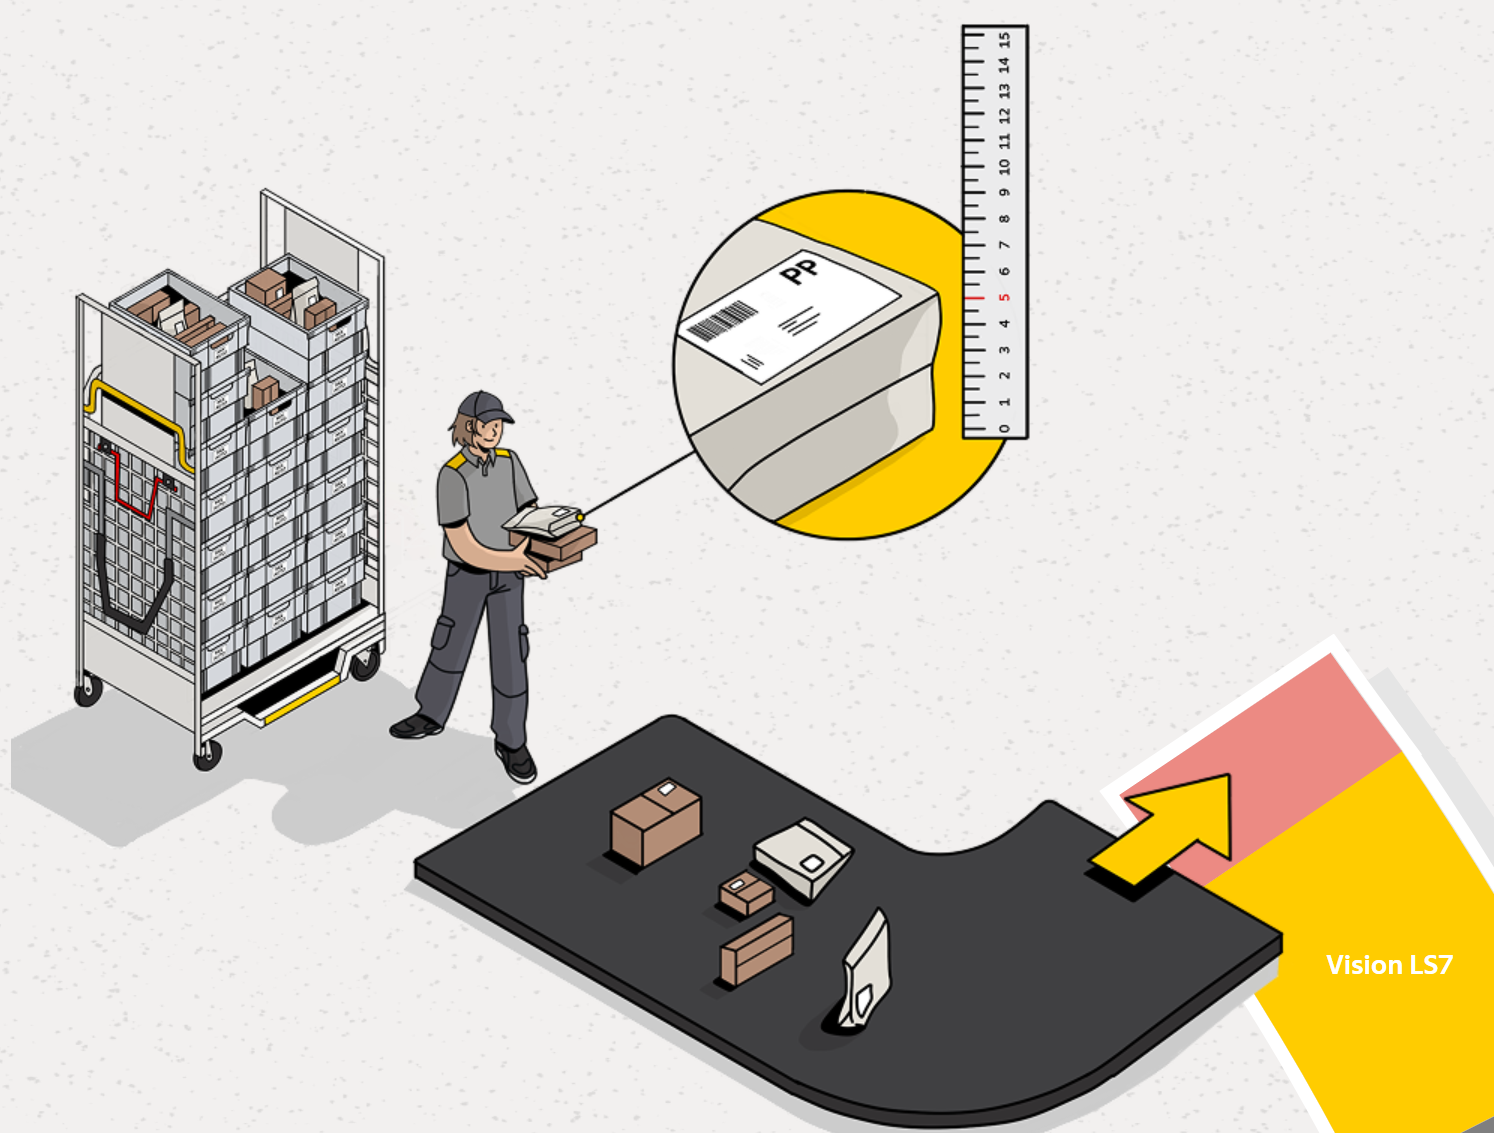
\includegraphics[width=0.8\textwidth]{./content/img/Post_internal/Visual_Subm1_PostGraphic_02_12_2025.png}
    \caption{Parcel sorting, smaller items submitted manually}
    \label{fig:submitting_small_manual}
\end{figure}
\begin{figure}[H]
    \centering
    \includegraphics[width=0.8\textwidth]{./content/img/Post_ExperienceHub/_DSC4856.jpg}
    \caption{Manual parcel onloading from a truck}
    \label{fig:Solution_manual_truck_unload}
\end{figure}

\subsubsection*{Discharged event}
\label{SolutionDischargedEvent}
The discharged event is complementary to the submitted event. It is the last automatic scan event of a parcel when it leaves the automated sorting machine. This can happen in different ways, such as when the parcel is discharged via a chute where staff load it into an RX, when it is discharged directly into an RX automatically by the machine, or when it is automatically ejected after completing a defined number of cycles through the machine. All of these possibilities trigger different follow-up actions. However, in all mentioned cases, a discharged scan is performed after the parcel is removed from the automatic sorting machine. This is the important aspect for reporting, as these two events (submitted and discharged) occur once per complete cycle that a parcel runs through the automatic sorters.

\begin{figure}[H]
    \centering
    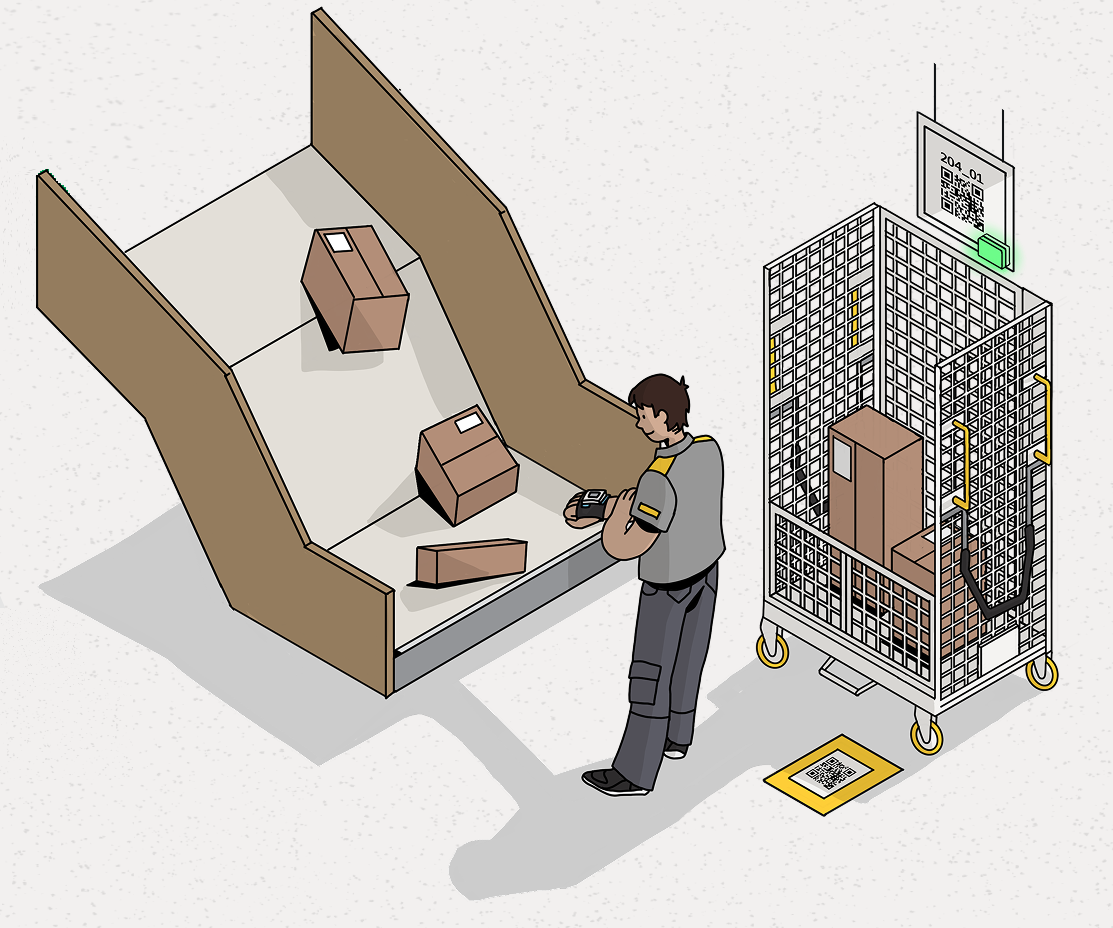
\includegraphics[width=0.8\textwidth]{./content/img/Post_internal/Visual_DisCh_PostGraphic_02_12_2025.png}
    \caption{Parcel discharged, manual loading into RX}
    \label{fig:discharged_manual_visualisationl}
\end{figure}



\section{Data Lineage}
\label{SolutionDataLineage}

The data relevant to this project are those used by the DWH LS OPS team. They consist of cleaned and deduplicated data stored in the \gls{curated} database layer. However, these data originate from sensor data and arrive in the data warehouse (\gls{DWH}) in a raw format. Before reaching the curated layer, the data pass through four main processing steps, which are also shown in the following figure:

\begin{itemize}
    \item \textbf{Physical data source}: Parcels are scanned by different scanners in the sorting centres. As described above, Swiss Post uses a variety of devices from different hardware vendors, which naturally results in a large number of data entities that must be stored. Each parcel passes through multiple scanners during its journey across the Swiss Post's 13 sorting centres, generating multiple data entities that are transferred to the data warehouse. Determining the exact number of generated events was outside the scope of this project.
    \item \textbf{Initial data storage}: The scan events are first saved in AWS S3.  At first glance this might be a very unusual choice, but the reasons make sense. First, the Swiss Post has a cloud strategy which includes AWS as a service provider; hence the choice of AWS is no surprise.  But more importantly, Amazon S3 (Simple Storage Service) is the object storage service of AWS. Exactly which data are stored here and how is addressed in a following section.
    \item \textbf{Kafka ingestion}: Apache Kafka is an open-source distributed event streaming platform designed for high-throughput, fault-tolerant, real-time data pipelines and event-driven architectures.The Swiss Post 
[ operates a Kafka environment in its down data centers ]
[ uses the Amazon MSK Managed Streaming for Kafka ].
With this,  so-called “producers” read the data from the initial storage and ingest it into Kafka “topics,” to which other systems can “subscribe” and obtain the data.

    \item \textbf{Data delivery to DWH}: Kafka consumers ingest the events into the DWH LS OPS raw data layer. Which is the first storage layer in this teams AWS S3 account, saving the data as recieved from Apache Kafka. 
\end{itemize}

\begin{figure}[H]
    \centering
    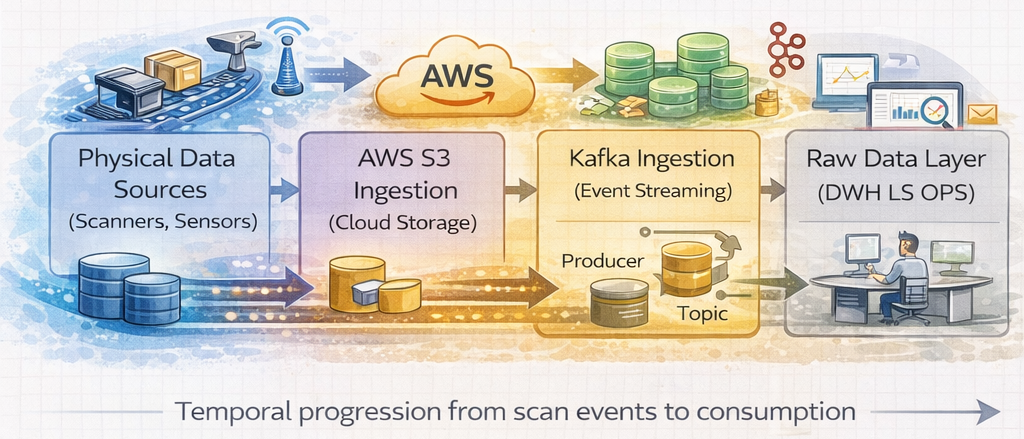
\includegraphics[width=0.8\textwidth]{./content/img/Solution_Design/DataLineage_ChatGPT_generated_MainSteps.png}
    \caption{An artistic high-level view of the DWH LS OPS data lineage}
    \label{fig:design_Datalineage_paintedGPT_beforeDWH}
\end{figure}

\textbf{KEY POINT:}  From the data creating stage until  the data arrives at the DWH, it passes through four IT system steps discussed here. This results in four potential sources of failure, in which each system is counted only once and by ignoring different possible errors per step. This landscape makes it difficult to trace errors that can occur at any step. Additionally, the variety of errors is large, as they may alter data values or result in no data being transmitted at a given step, even though the operation of the sorting center itself continues without issues. Therefore, at a technical level, providing clarity especially during the operational aspect is an important key aspect of this project.

Finally, to complete the picture of the data lineage, one more step is relevant. After the data has arrived in the raw layer at DWH LS OPS, it must be cleaned and deduplicated. At this step, differences in hardware providers and the structural differences of sorting centers come into effect, and the unification of the data takes place. All of this is performed in the step towards the curated database layer, after which a reporting layer serves as the final layer from which reporting tools retrieve data as introduced in chapter \ref{subsec:ResearchReportingPipeline}. This is illustrated here with a focus on the central step from the raw layer to the curated layer. Even after the curated layer, there is one additional layer, namely the reporting layer. 

The different layers in the cloud are set up according to a structure similar to that used in the classical on-premises DWH at Swiss Post. This similarity to the on-premises DWH stems from deliberate architectural alignment. The cloud infrastructure was built with the guidance of on-premises developers using their domain knowledge. In this way, functional and structural consistency was maintained, as the architecture continues to follow the Kimball star schema and the layered architecture as defined in the Kimball technical architecture \cite{KimballTechnicalArchitecture}.

\begin{figure}[H]
    \centering
    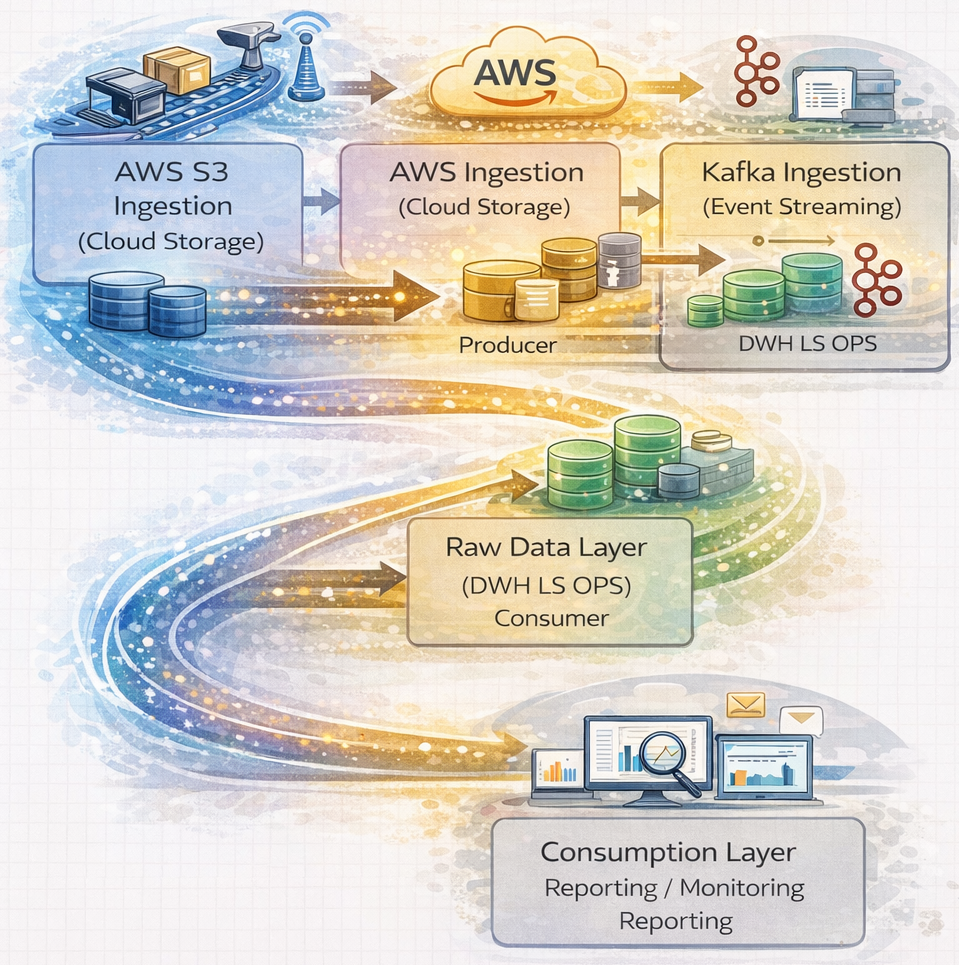
\includegraphics[width=0.8\textwidth]{./content/img/Solution_Design/DataLineage_ChatGPT_completer_view.png}
    \caption{An artistic high-level view of the full DWH LS OPS data lineage up to reporting}
    \label{fig:design_Datalineage_paintedGPT_full_tillReporting}
\end{figure}


\section{This project as a key step towards the “future state” reporting solution}
\label{SolutionIntentedSol}

As stated earlier the solutional goal of this project and its follow up is to provide an MVP for DQM, from which the key learnings will enable the full “future state” reporting solution. This MVP should implement an automatic data quality check, replacing an occasional, non automated check performed by the business. This is important, as the DQM check is currently executed by the business instead of IT, which creates challenges with regard to the desired target state. The expected situation would be that IT executes data quality checks and defines thresholds together with the business. At present, however, the knowledge about thresholds and other relevant information resides solely with the business.

In summary, having IT run the data checks would enable continuous follow-up of data quality. For example, a report based on automatically executed checks could show system uptime over a longer period of time. This information would later allow IT to extrapolate standard value ranges, which in turn would enable the definition of alerting thresholds. In short, having DQM checks executed automatically rather than occasionally by the business provides multiple benefits for both IT and the business.

\begin{figure}[H]
    \centering
    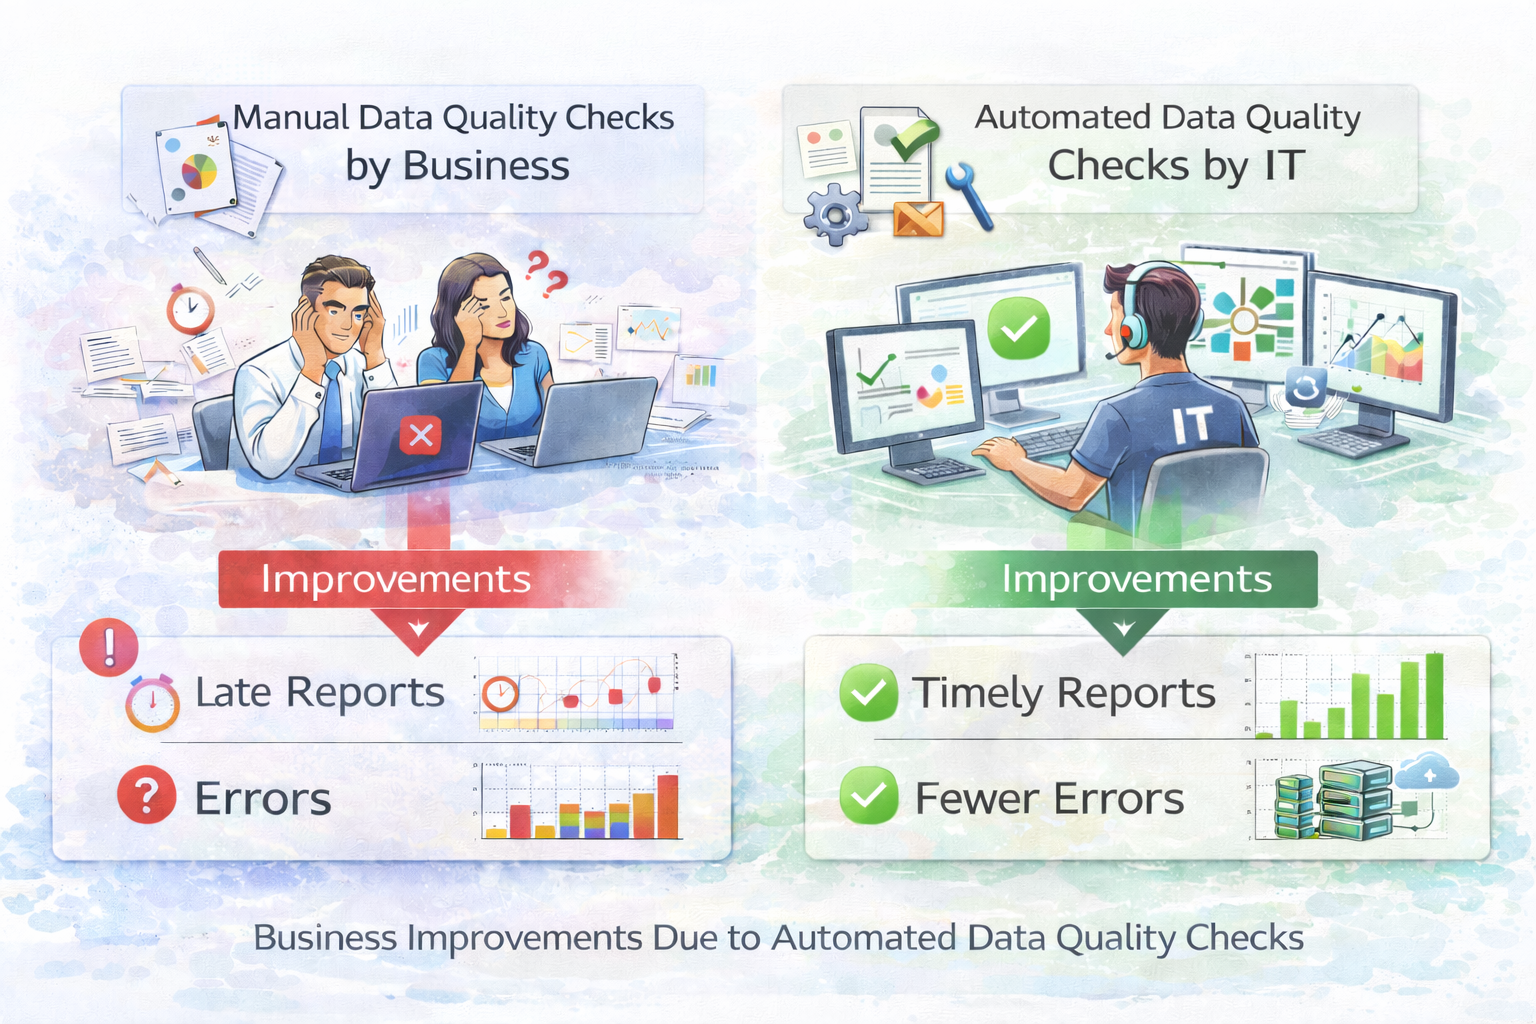
\includegraphics[width=0.8\textwidth]{./content/img/Solution_Design/businessChecks_against_ITautomated.png}
    \caption{DQM manual checks against automated checks by IT}
    \label{fig:dqm_manual_automated}
\end{figure}


\section{Expected benefits of this reporting solution}
\label{SolutionReasonsForSol}
A single visualisation does not explain the full benefit of the intended solution. For instance, the question arises as to why the business should stop performing data quality checks when it has the most detailed knowledge of the data. This is quickly clarified by taking a step back. The question should not be why checks are removed from the business, but why the reports are performed by the business in the first place. The benefits of this shift are therefore outlined in more detail in the following.

\subsection*{Benefit 1: Automation over manual processes to reduce effort}
\label{SolutionReasonsAutomationOverManual}
The business currently spends 30 to 45 minutes per day on a single data quality check, according to the initial project hand in description. From the duration of the check, it can be inferred that anyone requiring the data quality check before a report based on it is approved must wait until it is finished, resulting in a waiting time of 30 to 45 minutes. This fact provides the basis for understanding why manual processes are not suitable at scale. When scaling up to ten data quality checks, five to seven and a half hours are spent by the business on data quality checks. The waiting time for the last reports to be approved increases accordingly to five to seven and a half hours. When increasing to 20 checks per day, ten to 15 hours are spent, and the waiting time rises accordingly, accounting for more than one full-time position and long delays in report data release. It should be noted that this amount of time is spent solely to determine whether the defined check passes or not.
If the same initial check is executed by an automated data quality process, the expectation is that execution takes less than one minute; for simplicity, an execution time of one minute is assumed. As no manual initiation is required, no human time is spent performing the check. For comparison, the one minute waiting time for report approval and release is still considered. The business can then be informed whether the check returned an OK or not OK result, and the outcome can be stored for future reference.

When scaling this approach to ten checks, the total execution time remains ten times one minute. However, as the IT system can execute these checks in parallel, the waiting time for results remains at one minute. When increasing to 20 checks per day, the IT systems likewise execute the checks in parallel, and the execution and waiting time remain unchanged.

\subsubsection*{Benefit 2: Scalability to further reduce overall time required}
In summary, manual data quality checks cannot be scaled and lead to excessive use of human resources for repetitive tasks, as well as long waiting times for approved datasets. Automated data quality checks, by contrast, allow many checks to be executed in parallel within the same overall time frame. It should be noted that this comparison assumes all checks have similar complexity.

\subsection*{Benefit 3: Rule changes without query changes}
The current manual reports, which are business driven, have their logic built directly into the queries executed on the data. If any rule changes or a part of the data processing is modified, these queries need to be adapted. Thus, the check is deeply tied to the data source. To illustrate this with an example, a data quality check may confirm that 30\% of the data is category A and 70\% is category B, as this is considered the expected and valid distribution. If changes to processing pipelines or client behaviour cause the share of A to increase to 45\% and B to decrease to 55\%, the query performing the check must be adapted. However, when the check is performed by an application that injects these thresholds into a query, the query itself does not need to change, and only the parameters must be adjusted.

\subsubsection*{Benefit 4:  Reusability to improve stability and performance}
By moving the responsibility for checks from manual, business-driven processes to automated checks executed by IT, the checks can be designed to be more generic. Generic checks can be reused across different use cases. This separation of responsibilities and concerns leads to improved stability and performance when applying the checks, which in turn enables strong reusability. The same check type can be applied to different data sources by adapting parameters such as the query and thresholds, while the underlying check logic remains unchanged.



\section{Existing reporting pipeline}
\label{SolutionReportingPipeline}
The current reporting pipeline at DWH LS OPS team consists of four main components as shown in following figure and introduced in chapter \ref{subsec:ResearchReportingPipeline}. First, the storage layer (in figure : \textbf{Datenspeicherung}), where data is retrieved, cleaned, and saved to \gls{AWSS3}. Second, the query and processing layer, where cleaned data is queried using Amazon \gls{athena} and \gls{DSP}(in figure : \textbf{Datenselektierung, Datenpreparation Datenmodelle Data Federation}), and where data is passed and persisted in data models for reports. Third, the reporting and consumption layer, in which data from DSP is used in \gls{SAC} reports (in figure : \textbf{Business Layer}).

\begin{figure}[H]
    \centering
    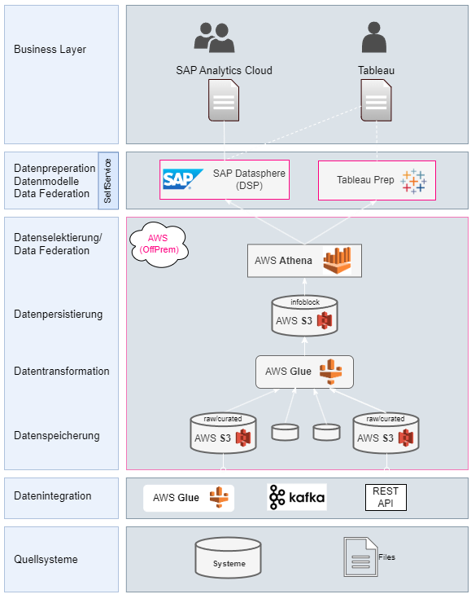
\includegraphics[width=0.8\textwidth]{./content/img/Solution_Design/DWH_CloudSTructure_OnlyHW.png}
    \caption{The DWH LS OPS reporting layers}
    \label{fig:Solution_Landscape_cloud_layers}
\end{figure}

\subsubsection*{AWS S3}

As described by Amazon: \textit{“Amazon Simple Storage Service (Amazon S3) is an object storage service that offers industry-leading scalability, data availability, security, and performance. Customers of all sizes and industries can use Amazon S3 to store and protect any amount of data for a range of use cases, such as data lakes, websites, mobile applications, backup and restore, archive, enterprise applications, IoT devices, and big data analytics. Amazon S3 provides management features so that you can optimize, organize, and configure access to your data to meet your specific business, organizational, and compliance requirements.” \cite{aws_s3_docs}.}

This is relevant for Swiss Post, as Amazon S3 serves as the central storage for data from mail piece events, which include all scans of parcels and mail in sorting centers, as well as later stages up to the delivery process. This storage is used by the DWH LS OPS team. All data entering the data lineage pipeline, for example through Kafka or through direct database connections, is stored in Amazon S3. Thus, it represents the first persistence point in the reporting pipeline.

\paragraph{Layered architecture}
It is important to note that the data is not only initially saved to Amazon S3 in a raw layer, but is also cleaned and prepared for reporting in two additional layers. To separate the storage of raw data from the cleaning process, multiple layers are used. This ensures that all data in its original format is saved first before processing, modification, augmentation, and checks for completeness or correctness are performed. Each step can therefore be reproduced and repeated, which is useful whenever data needs to be reloaded, for example when data was incomplete for a day or when new processing methods are developed.
After the raw layer, data is deduplicated and cleaned, and then saved into the curated layer. The final top layer, the reporting layer, mainly adds translations of fields into business terminology, for example by changing column labels. This is useful for the business, as it enables consistent naming of columns across tables or data products. 

\paragraph{Infoblock}
\label{SolutionLandscapeInfoblock}
On this level \gls{infoblock}'s are generated, this is a Swiss Post internal term used for report ready data products. An infoblock is cleaned, deduplicated, curated data which features joined datasets that use business naming, e.g. \gls{postday} and processing, priority types. Basically the infoblocks are the final layer employed on the reporting layer, making them accessible to the reporting tools such as \gls{DSP} and \gls{SAC}, which are described in detail below. A more comon term for infoblock know trough out the industry is data product  \cite{alation_data_product, ibm_data_product}. 

\subsubsection*{AWS Athena query}
\label{SolutionAthenaQuery}
The next step is Amazon Athena as the query layer, which Amazon describes as follows: \textit{ “Amazon Athena is an interactive query service that makes it easy to analyze data directly in Amazon Simple Storage Service (Amazon S3) using standard SQL. With a few actions in the AWS Management Console, you can point Athena at your data stored in Amazon S3 and begin using standard SQL to run ad-hoc queries and get results in seconds. “ \cite{aws_athena_docs}.}
Amazon Athena is used by Swiss Post DWH LS OPS for all queries on Amazon S3, which is the next step in the reporting pipeline. Athena is the tool designed by AWS for use with S3, making it the logical choice for querying the stored data. The data is queried for reporting purposes by selecting the relevant subsets.

\paragraph{DQM relevance}
The querying layer is relevant to DQM, since data quality issues may become apparent first at this earliest checkpoint, for example when errors occur in the data itself and counts or joins become invalid. While the data is queried at this layer for reporting purposes, it is also queried here for data quality checks. Such checks typically address missing data and data completeness, but can also extend to data plausibility, for example when postal codes are compared to cities. In cases where issues occur at this layer, they are passed downstream towards DSP and SAC, provided they do not already break the pipeline at this stage.


\subsubsection*{SAP products SAP Datasphere (DSP) and SAP Analytics Cloud (SAC)}
At Swiss Post, the next step in the reporting pipeline uses the two dependent tools SAP Datasphere (DSP) and SAP Analytics Cloud (SAC). These are described as follows by SAP:

\textit{SAP Datasphere enables organizations to combine, harmonize, and model data from multiple SAP and non-SAP sources within a semantically rich, cloud-based data environment. 
SAP Analytics Cloud can directly consume these governed and business-ready data models via live connections, enabling interactive reporting, analytics, planning, and forecasting. 
In addition, planning and forecast data created in SAP Analytics Cloud can be written back to SAP Datasphere, allowing analytical and planning data to coexist in a single, integrated data foundation \cite{sap_datasphere_sac_integration}.}

SAP Datasphere (DSP) is SAP’s cloud-based data platform for integrating, modeling, and analyzing data across SAP and non-SAP systems while preserving business semantics. It enables federated access to distributed data without full replication and supports end-to-end data lineage and governance. DSP at Swiss Post is used as the analytical backbone for reporting, analytics, and data-driven decision-making in SAP landscapes.

SAP Analytics Cloud (SAC), in turn, uses the data model provided by DSP to present this information on the business layer to end users. More information on this is provided in the separate section introducing the tool.


\subsubsection*{DSP datamodel}
\label{SolutionDesignDSPModel}
After querying, the data is persisted in \gls{DSP}, where it is made available in data models. This persistence and processing layer is essential in the current pipeline, as data can be made available to \gls{SAC} only through DSP. At Swiss Post, data persistence has proven essential to improving the response time of the reporting pipeline as a whole.
 With this persistence, DSP does not pass queries back to Amazon Athena, creating a clear separation between the two layers. Due to this separation, DSP is not responsible for DQM, which is handled in lower layers. Finally, DSP is the layer in which business logic is applied in a semantic form, defining what the data represents. At Swiss Post, this is done by applying business oriented naming and calculations. Different report consumers may require the same values to be structured in different ways; for example, productivity in a sorting center may be measured using total working hours against the number of mail pieces handled, or calculated using only time spent on sorting-related tasks, excluding breaks, training, and other activities.
 
\paragraph{DSP use case}
The data models in DSP are useful not only as a bridge to SAC (discussed below). They allow different data sources to be modelled and combined into unified data models. This is also relevant to Swiss Post, as it operates not only Amazon Athena data sources but also other database- or file-based sources. This combination of data inevitably inherits data quality issues from the underlying sources, which can affect joins, data loading, and further processing. Nonetheless, DSP is the sole source of data provided to SAC, which is the next logical step in the reporting pipeline. This also means that any unhandled data quality issues are passed directly to users consuming reports in SAC and may therefore affect confidence in the reporting pipeline depending on data quality.

\subsubsection*{SAP Analytics Cloud (SAC) report}
SAC is the final step in the reporting pipeline and represents the reporting and consumption layer. As the last layer, it inherits the data from previous layers and is responsible only for its visualisation. The data is displayed passively, and no further transformations are performed at this stage. Consequently, any errors in data preparation or data quality issues from upstream layers are propagated to this layer together with the data itself.

As described earlier, SAC is dependent on DSP and cannot operate independently, nor does it provide native DQM capabilities. The reports generated by SAC are therefore fully dependent on the preceding layers, and any issues or delays are reflected directly in the reports. This is particularly relevant for Swiss Post, as one report provided by DWH LS OPS is used daily at 07:00 for shift handover, which takes place one hour after the end of the \gls{postday}. Some data sources required for this report become available only after 06:00, the end of the postday. If any upstream step is delayed, the report delivery is delayed accordingly.

\paragraph{Consumption layer}
As the consumption layer for reports, this is the point at which users with read access have their first and only interaction with the reporting pipeline. It is at this stage that user confidence is either established or lost, making it particularly critical. Users do not see the upstream processing steps and typically do not differentiate whether missing or delayed information is caused by AWS S3, Athena, or DSP.